\begin{figure*}[t]
\centering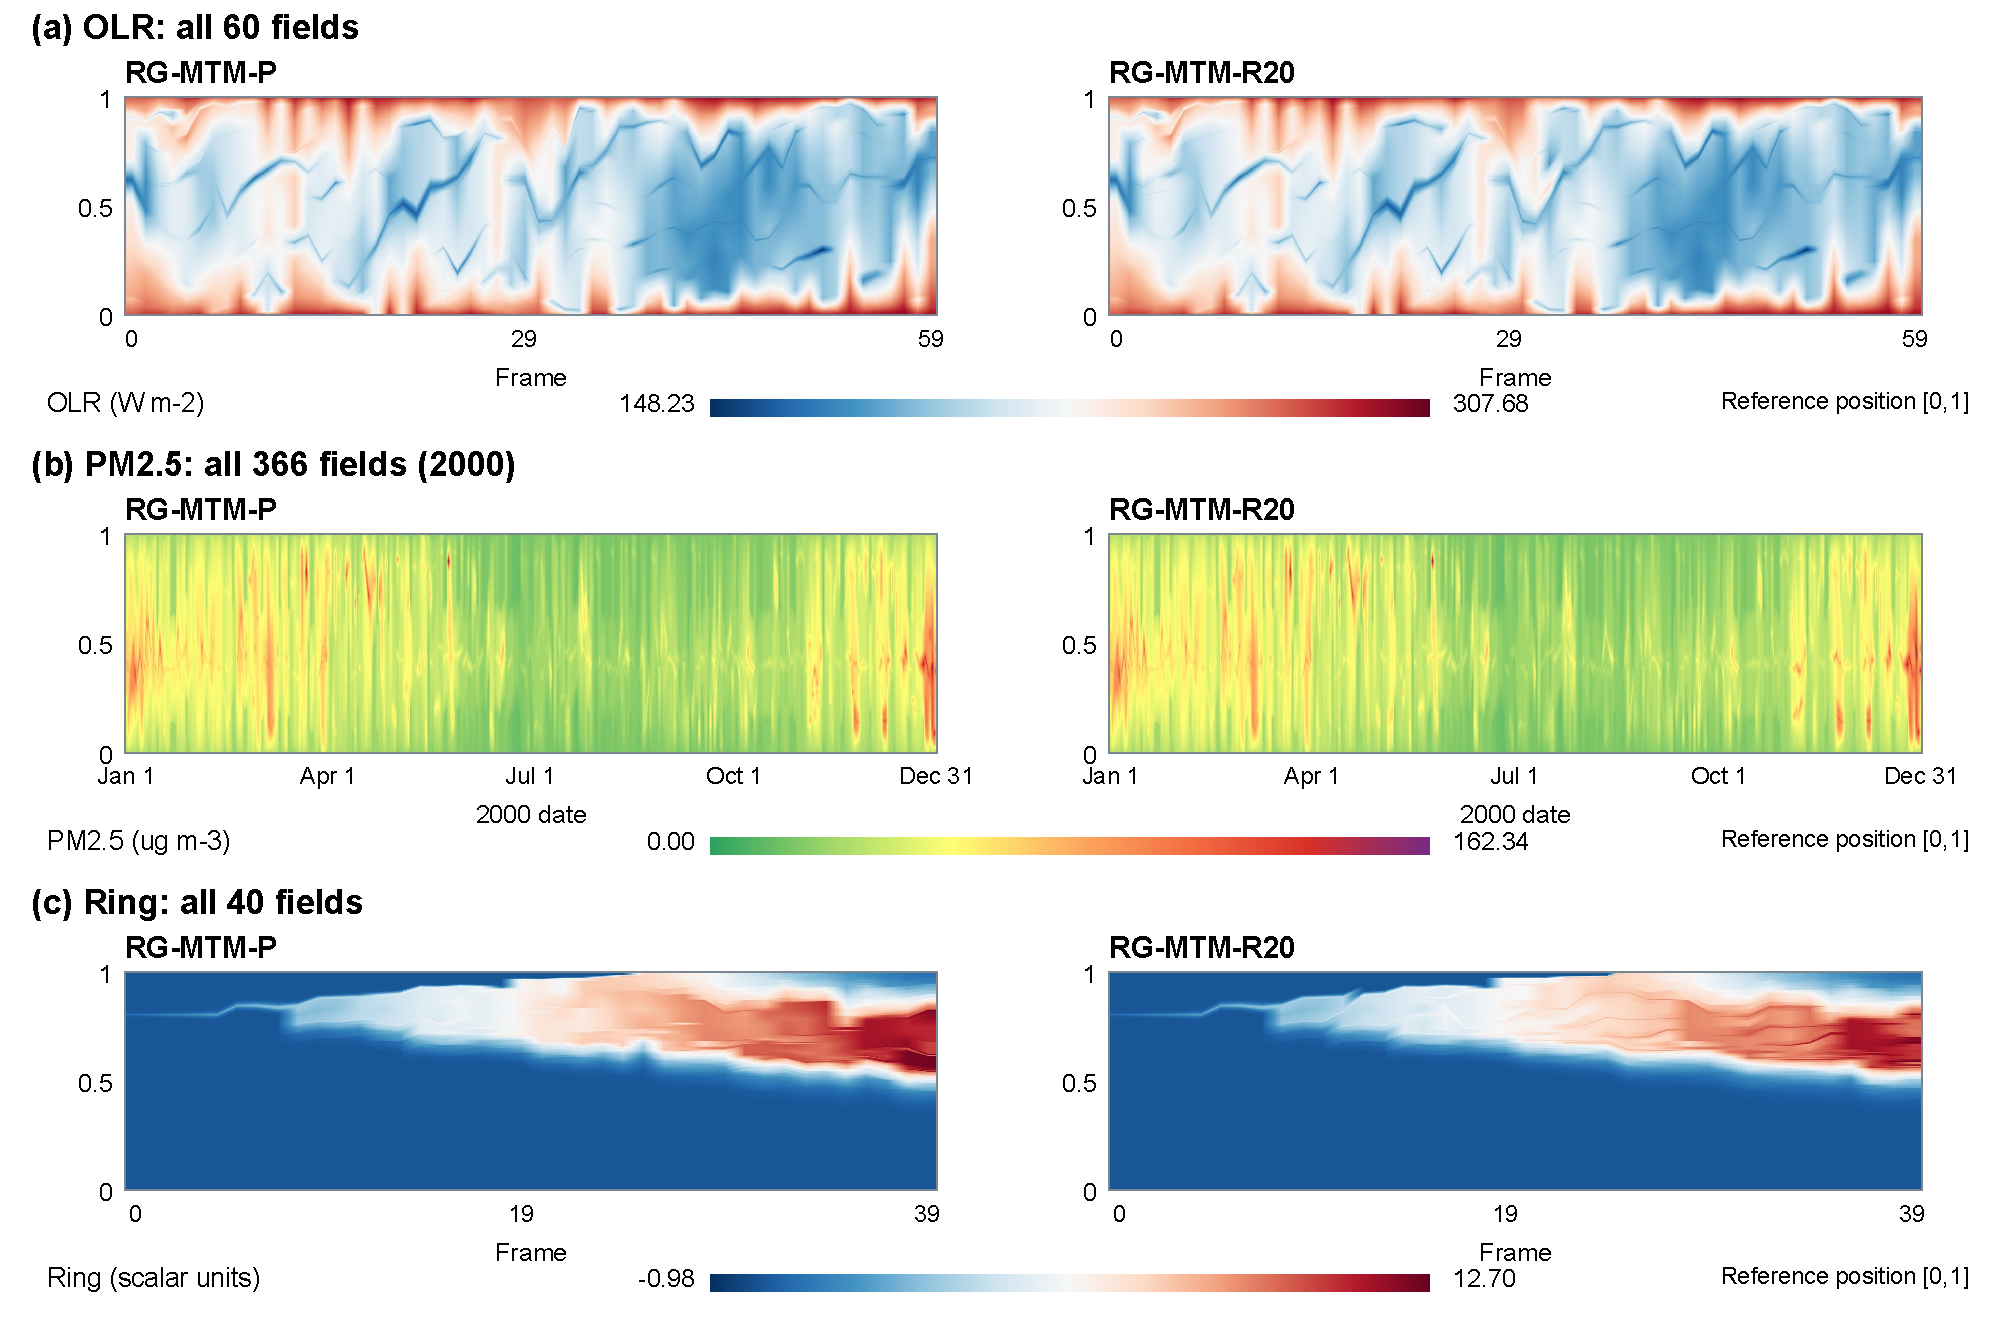
\includegraphics[width=\textwidth]{figures/Fig12.pdf}
\caption{Complete P/R20 temporal maps for three additional inputs: (a) OLR, all 60 daily fields; (b) PM2.5, all 366 fields in 2000; (c) Ring, all 40 synthetic fields. Horizontal axes show frames; vertical axes show the same normalized fixed reference within each P/R pair. Scalar ranges are shared within each row and independent between datasets. Maps use complete sequences without temporal cropping. Conservative display interpolation preserves each saved profile exactly; intermediate columns do not add observations. PM2.5 uses the user-authorized green--yellow--orange--red--purple pollution palette in concentration units, without AQI thresholds. Colours encode processed scalar values; any below-input-range connections are layout outputs. Complete arrays, not preview pixels, determine the reported errors. The complete four-method comparisons are in Supplement S10.}
\label{fig:remaining_temporal}
\end{figure*}
